\section{Theorie}
\label{sec:theorie}

    Im folgenden Abschnitt werden die theoretischen Grundlagen eines Fadenpendels erläutert.\\
    \\
    Zuerst wird ein einfaches Fadenpendel der Länge l und einer Masse m betrachtet,
    welches möglichst reibungsfrei schwingt.
    Die Bewegung des Pendels nach einer kleinen Auslenkung aus der Ruhelage um den Winkel $\phi$ lässt sich mit der Gleichung
    \begin{equation*}
        J \cdot \ddot{\phi} + D_\text{p} \cdot \phi = 0
        \label{eqn:dgl_einzelpendel}
    \end{equation*}
    beschreiben,
    wobei in diesem Fall die Kleinwinkelnäherung 
    \begin{equation}
        \sin{\phi} \approx \phi
        \label{eqn:kleinwinkelnaeherung}
    \end{equation}
    gilt.
    Die Produkt $D_\text{p} \cdot \phi$ beschreibt das Drehmoment $M$,
    welches auf das Pendel wirkt,
    wenn es ausgelenkt wird.
    Das Drehmoment entsteht durch die Gewichtskraft $\vec{F} = m \cdot \vec{a}$,
    welche der Auslenkung entgegenwirkt.
    Der Faktor $D_\text{p}$ beschreibt die Winkelrichtgröße des Pendels.
    Zusätzlich hat das Trägheitsmoment $J$ des Pendels einen Einfluss auf die Bewegung.\\
    Das Pendel schwingt nach der Auslenkung harmonisch,
    was bedeutet,
    dass es um seine Ruhelage oszilliert und vollständig durch eine Sinus- oder Kosinusfunktion beschrieben werden kann.
    Aus der Lösung der Differentialgleichung \eqref{eqn:dgl_einzelpendel} kann die Schwingungsfrequenz
    \begin{equation*}
        \omega = \sqrt{\frac{D_\text{p}}{J}} = \sqrt{\frac{g}{l}}
    \end{equation*}
    bestimmt werden.\\
    \\
    Im Folgenden werden zwei Pendel gleicher Länge und Masse betrachtet,
    welche durch eine Feder gekoppelt sind.
    Durch die Kopplung wirken zusätzliche Drehmomente $M_1 = D_\text{F}(\phi_2 - \phi_1)$ und $M_2 = D_\text{F}(\phi_1 - \phi_2)$ auf die Pendel.
    Ihre Bewegung lässt sich mit gekoppelten Differentialgleichungen darstellen,
    bei denen die linke Seite die Bewegung des jeweiligen Pendels,
    und die rechte Seite die Kopplung beschreibt.
    Es gilt
    \begin{gather*}
        J \ddot{\phi_1} + D \phi_1 = D_\text{F}(\phi_2 - \phi_1) 
        \label{eqn:dgl1_kopplung}\\
        J \ddot{\phi_2} + D \phi_2 = D_\text{F}(\phi_1 - \phi_2) \ .
        \label{eqn:dgl2_kopplung}
    \end{gather*}
    Bei der Entkopplung der Schwingungen wird eine Überlagerung aus Eigenschwingungen mit den Auslenkwinkeln $\alpha_1$ und $\alpha_2$ beschrieben.
    Abhängig von den Anfangsbedingungen der Auslenkung $\alpha(t=0)$ und $\dot{\alpha}(t=0)$ können zwischen gleichsinnigen,
    gegensinnigen und gekoppelten Schwingungen unterschieden werden.

\subsection{Gleichsinnige Schwingungen}
\label{sec:gleichsinnige_schwingung}

    Die beiden Pendel werden,
    wie in Abbildung \ref{fig:gleichsinnig} dargestellt,
    um den gleichen Winkel $\alpha_1 = \alpha_2$ ausgelenkt,
    sodass nur die Gewichtskraft als rücktreibenden Kraft wirkt.
    Die Verbindung der Pendel über die Feder hat keinen Einfluss auf die Schwingung,
    weshalb die Feder entfernt werden kann.
    Für die Schwingungsfrequenz ergibt sich
    \begin{equation}
        \omega_+ = \sqrt{\frac{g}{l}} \ ,
        \label{eqn:frequenz_gleichsinnig}
    \end{equation}
    wobei $g$ die Erdbeschleunigung darstellt.
    Die Schwingungsdauer $T$ ergibt sich aus dem Zusammenhang $\omega = \frac{2\symup{\pi}}{T}$ 
    \begin{equation}
        T_+ = 2\symup{\pi} \sqrt{\frac{l}{g}} \ .
        \label{eqn:dauer_gleichsinnig}
    \end{equation}

    \begin{figure} 
        \centering
        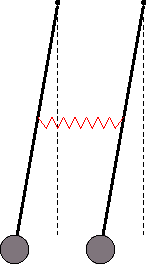
\includegraphics[scale=0.9]{content/img/Abb_1.pdf}
        \caption{Darstellung der gleichsinnigen Schwingung bei zwei gekoppelten Pendel.}
        \label{fig:gleichsinnig}
    \end{figure}

\subsection{Gegensinnige Schwingungen}
\label{sec:gegensinnige_schwingung}

    Beide Pendel werden um den gleichen Winkel $\alpha_1 = -\alpha_2$ in entgegengesetzte Richtungen ausgelenkt,
    sodass die Feder eine gleich große,
    rücktreibende Kraft ausübt,
    siehe Abbildung \ref{fig:gegensinnig}.
    Für die Schwingungsfrequenz ergibt sich
    \begin{equation}
        \omega_- = \sqrt{\frac{g}{l} + \frac{2K}{l}}
        \label{eqn:frequenz_gegensinnig}
    \end{equation}
    mit der Kopplungskonstante $K$ der Feder.
    Für die Schwingungsdauer ergibt sich 
    \begin{equation}
        T_- = 2\symup{\pi} \sqrt{\frac{l}{g + 2K}} \ .
        \label{eqn:dauer_gegensinnig}
    \end{equation} 
    \begin{figure}
        \centering
            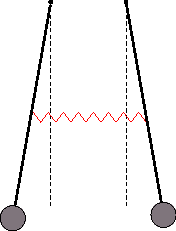
\includegraphics[scale=0.9]{content/img/Abb_2.pdf}
            \caption{Darstellung der gegensinnigen Schwingung bei zwei gekoppelten Pendel.}
            \label{fig:gegensinnig}
    \end{figure}
    
    
    Die Kopplungskonstante $K$ wird als Maß für die Kopplung betrachtet und kann aus den folgenden Zusammenhängen berechnet werden.
    \begin{equation}
        K = \frac{\omega^2_- - \omega^2_+}{\omega^2_- + \omega^2_+} = \frac{T^2_+ - T^2_-}{T^2_+ + T^2_-} 
        \label{eqn:kopplungskonstante}
    \end{equation}

\subsection{Gekoppelte Schwingungen}    
\label{sec:gekoppelte_schwingung}   
        
    Ein Pendel bleibt zu Beginn in seiner Ruhelage $\alpha_1 = 0$,
    während das andere um den Winkel $\alpha_2 \neq 0$ ausgelenkt wird.
    Durch die Feder kann das schwingende Pendel seine Energie auf das ruhende Pendel übertragen und es so zum Schwingen anregen,
    wie in Abbildung \ref{fig:gekoppelt} gezeigt.
    Dabei sinkt die Auslenkung des ersten Pendels und die des zweiten Pendels nimmt solange zu,
    bis sich das erste Pendel in Ruhe befindet und das zweite Pendel maximal ausgelenkt wird.
    Der Zeitraum,
    in dem ein Pendel aus seiner Ruhelage heraus angeregt wird und schließlich wieder dorthin zurückkehrt,
    wird als Schwebung bezeichnet.
    Für die Schwebungsfrequenz ergibt sich
    \begin{equation}
        \omega_\text{S} = \omega_+ - \omega_-
        \label{eqn:frequenz_schwebung}
    \end{equation}
    und für die Schwebungsdauer
    \begin{equation}
        T_\text{S} = \frac{T_+ \cdot T_-}{T_+ - T_-} \ . 
        \label{eqn:dauer_schwebung}
    \end{equation}
    Der Vorgang der vollständigen Energieübertragung setzt sich periodisch fort.
    \begin{figure}
        \centering
            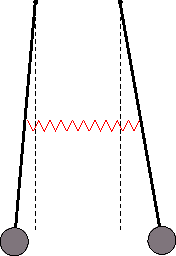
\includegraphics[scale=0.9]{content/img/Abb_3.pdf}
            \caption{Darstellung der gekoppelten Schwingung bei zwei gekoppelten Pendel.}
            \label{fig:gekoppelt}
    \end{figure}
